\begin{appendices}

\section{Stability}\label{sec:stability}

\Cref{fig:compare} shows the blow up of the numerical solution with forward
time step with $\Delta t = 1$ and $\Delta x = 0.025$ for the periodic case.
With a central difference in time the solution seems stable.

\begin{figure}[h]
  \centering
  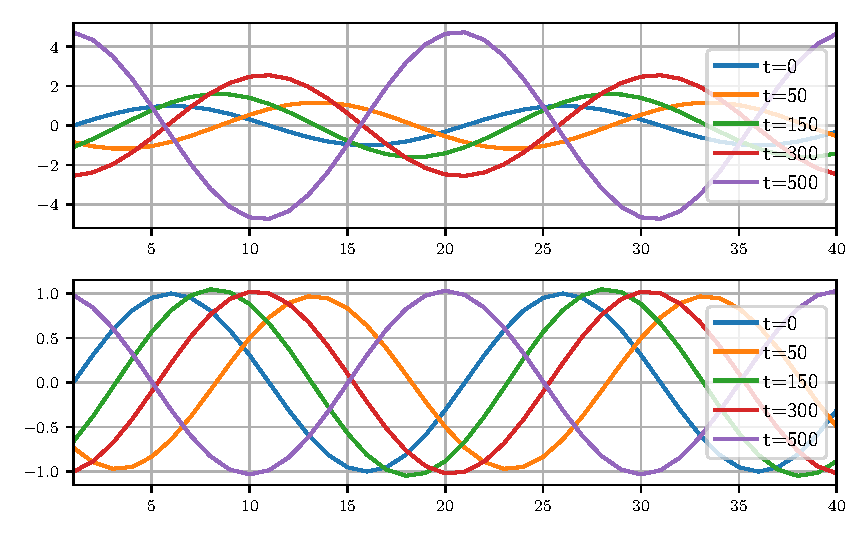
\includegraphics[width=\textwidth]{../figures/compare_dt_1.pdf}
  \caption{Comparison of solutions with periodic boundaries
  at different times using forward (top) and
  centered (bottom) differences in time with $\Delta x$ = 0.025 and $\Delta t$
  = 1. The solution using forward differences
  blows up quickly while the one using central differences does not.}
  \label{fig:compare}
\end{figure}

\end{appendices}
